%! program = pdflatex

%\documentclass[12pt,a4paper]{memoir} % for a long document
%\documentclass[12pt,a4paper,article]{memoir} % for a short document


\documentclass[12pt,a4paper,article]{memoir}
\usepackage{geometry}
 \geometry{
 a4paper,
 left=20mm,
 right=20mm,
 top=20mm,
 bottom=20mm,
 }
% \usepackage[titletoc]{appendix}

\usepackage{graphicx}
\usepackage{listings}
\usepackage[dvipsnames]{xcolor}
\usepackage{hyperref}
\usepackage{cleveref}

\usepackage{paralist}
\setlength{\parskip}{0.5\baselineskip plus2pt minus2pt}
\setlength{\parindent}{0pt}

\usepackage{enumitem}
\setlist[enumerate]{itemsep=0pt,topsep=0pt}
\setlist[itemize]{itemsep=0pt,topsep=0pt}


%\lstset{frame=tb,
%  language=C++,
%  aboveskip=3mm,
%  belowskip=3mm,
%  showstringspaces=false,
%  columns=flexible,
%  basicstyle={\small\ttfamily},
%  numbers=none,
%  numberstyle=\tiny\color{mygray},
%  keywordstyle=\color{blue},
%  commentstyle=\color{mygreen},
%  stringstyle=\color{mymauve},
%  breaklines=true,
%  breakatwhitespace=true,
%  tabsize=2
%}

\definecolor{codegreen}{rgb}{0,0.6,0}
\definecolor{codegray}{rgb}{0.5,0.5,0.5}
\definecolor{codepurple}{rgb}{0.58,0,0.82}
\definecolor{backcolour}{rgb}{0.95,0.95,0.92}
 

\lstdefinestyle{MyCodeStyle} {
%  language=C++, % choose the language of the code
  backgroundcolor=\color{backcolour},
  commentstyle=\color{codegreen},
  keywordstyle=\color{magenta},
  numberstyle=\tiny\color{codegray},
  stringstyle=\color{codepurple},
  basicstyle=\footnotesize,
  breakatwhitespace=false,
  breaklines=true,
  captionpos=b, % sets the caption-position to bottom
  keepspaces=true,                 
  numbers=none, % where to put the line-numbers
  showspaces=false, % show spaces adding particular underscores
  showstringspaces=false, % underline spaces within strings
  showtabs=false, % show tabs within strings adding particular underscores
  frame=single, % adds a frame around the code
  tabsize=2, % sets default tabsize to 2 spaces
  rulesepcolor=\color{blue},
  rulecolor=\color{black},
  xleftmargin=.1\textwidth,
  xrightmargin=.1\textwidth,
}

\hypersetup{
    colorlinks,
    citecolor=black,
    filecolor=black,
    linkcolor=black,
    urlcolor=black
}

\graphicspath{ {./img/} }
% See the ``Memoir customise'' template for some common customisations
% Don't forget to read the Memoir manual: memman.pdf

\title{Optimizing Alya simulations of multi-physics problems with Dakota}
\author{Rogeli Grima}
%\date{10/12/2014} % Delete this line to display the current date

% Make appear "Appendix" in the ToC
\renewcommand*{\cftappendixname}{Appendix\space}

%%% BEGIN DOCUMENT
\begin{document}

\maketitle
\tableofcontents*

\chapter{Introduction}

Dakota is a toolkit that provides a flexible, extensible interface between analysis codes and iterative systems analysis methods. It contains algorithms for optimization, uncertainty quantification, parameter estimation and sensitivity/variance analysis.

Alya is a computational method that is used to simulate complex physical systems. On many occasions we want to use these simulations to find an acceptable or optimized solution for a particular system. Dakota will help us to use Alya as a design tool. It will help us to solve very important questions as: What is the best design? How safe is it? How much confidence do I have in my answer?

This user's guide is intended to provide some background information on how to use Dakota to solve optimization problems that involve a simulation with Alya. We assume the user has some familiarity with Alya execution and configuration.

In this guide we will show how to use Dakota in Marenostrum, how to prepare your simulations with Alya, how to process their outputs and we will provide some basic examples.

\section{Dakota workflow}

Before you start working with Dakota and Alya, is important to know the Dakota's workflow. This will give you a better perspective of what is happening.

Dakota receives input and configuration from a variety of text files prepared by the user, and connects to any simulation code by other text files. This simple interface is one of the most important features of Dakota, as it makes it easy to change the iterative method or strategy by just changing a few lines in the Dakota input file.

In Figure \ref{fig:Workflow}, we can see the Dakota workflow. The user should provide an input file to Dakota. This input file controls the algorithm that we want to run, the function to be evaluated, the variables of this function and the outputs that we expect.

\begin{figure}[htb!]
  \centering
    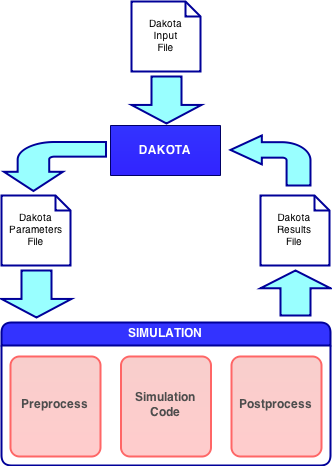
\includegraphics[width=0.4\textwidth]{DakotaWorkflow}
  \caption{Dakota Workflow}
  \label{fig:Workflow}
\end{figure}

Dakota generates a parameter file for every function evaluation. This file contains a specific value of every variable and specifies the kind of returning values that it needs (function evaluation, derivatives or/and second derivatives).

Dakota treats the simulation code as a black box. Most of the codes, like Alya, don't know what to do with the parameter file, so it is common to create a script to connect the simulation code with Dakota. In this script we merge the Dakota parameters file with the simulation code input files. Once we have some proper input files we can run the simulation code, extract the significant data from its output files and post-process that data in order to generate the appropriate objective function and the Dakota results file.

\chapter{Dakota tutorial}
\section{Set up Dakota}

We have installed in Marenostrum the last three versions of Dakota. Althought, most of the experiments that we have ran have been done using version 5.4 we encourage you to use the last version. From now on, all the information that we will provide you in this guide will refer to version 6.1. You can find the several installed versions of Dakota in:

\begin{itemize}
\item \textit{/gpfs/projects/bsc21/DAKOTA/dakota-5.4.0}
\item \textit{/gpfs/projects/bsc21/DAKOTA/dakota-6.0.0}
\item \textit{/gpfs/projects/bsc21/DAKOTA/dakota-6.1.0}
\end{itemize}

If you want to install your own version of Dakota in Marenostrum, please check Appendix \ref{chapter:CodeMod}.


In order to run Dakota you will need to set the path of the executables and the directory of the shared libraries. You can add these lines to your .barshrc file:

\begin{lstlisting}[style=MyCodeStyle,language=bash]
export DAK_INSTALL=/gpfs/projects/bsc21/DAKOTA/dakota-6.1.0
export PATH=${DAK_INSTALL}/bin/:${PATH}
export LD_LIBRARY_PATH=${DAK_INSTALL}/bin:${LD_LIBRARY_PATH}
export LD_LIBRARY_PATH=${DAK_INSTALL}/lib:${LD_LIBRARY_PATH}
\end{lstlisting}

Check that everything is working properly by running:

\begin{lstlisting}[style=MyCodeStyle,language=bash]
dakota -v
\end{lstlisting}

\section{Runing Dakota with a simple input file}
\label{section:RunDakota}

This section is intended for users who are new to Dakota, to demonstrate the basics of running a simple example.

\begin{enumerate}
\item Create a working directory.
\item From path \textit{/gpfs/projects/bsc21/DAKOTA/Examples/power}, copy files \textit{power\_multidim.in} and \textit{power.py} to the working directory.
\item From the working directory, run: \textit{dakota -i power\_multidim.in -o power\_multidim.out \textgreater{} power\_multidim.stdout}
\end{enumerate}

Dakota outputs a large amount of information to help users track progress. Four files should have been created:
\begin{enumerate}
\item The screen output has been redirected to the file power\_multidim.stdout. The contents are messages from Dakota and notes about the progress of the iterator (i.e. method/algorithm).
\item The output file \textit{power\_multidim.out} contains information about the function evaluations.
\item \textit{power\_multidim.dat} is created due to an specification of the input file. This summarizes the variables and responses for each function evaluation.
\item \textit{dakota.rst} is a restart file. If a Dakota analysis is interrupted, it can be often be restarted without losing all progress.
\end{enumerate}

This example used a parameter study method and the \textit{power.py} test problem. The Python script \textit{power.py} reads a Dakota parameters file, computes the function $F(x,y)=(X-0.5)^2+(Y+0.5)^2$ and writes the result in a Dakota results file.

As we said, this is a parametric study. Let's try to execute an optimization problem. Now, copy file \textit{power\_mas.in} to your working directory and run:

%dakota -i  power\_mas.in -o power\_mas.out \textgreater{} power\_mas.stdout
\begin{lstlisting}[style=MyCodeStyle,language=bash]
dakota -i  power_mas.in -o power_mas.out > power_mas.stdout
\end{lstlisting}

This executes a mesh adaptive direct search algorithm. If you look at the output file you will see that the method converges in 160 iterations and propose as a best objective function a value of $F(X,Y)=0.0$ evaluated for $X=0.5$ and $Y=-0.5$ . That is the minimum of the evaluated function.

You can see a graphic representation of the results executing the script \textit{visualize.sh} that you can find in the same directory. This scripts reads the results from the parametric study and from the mesh adaptive direct search algorithm.

\begin{figure}[htb!]
  \centering
    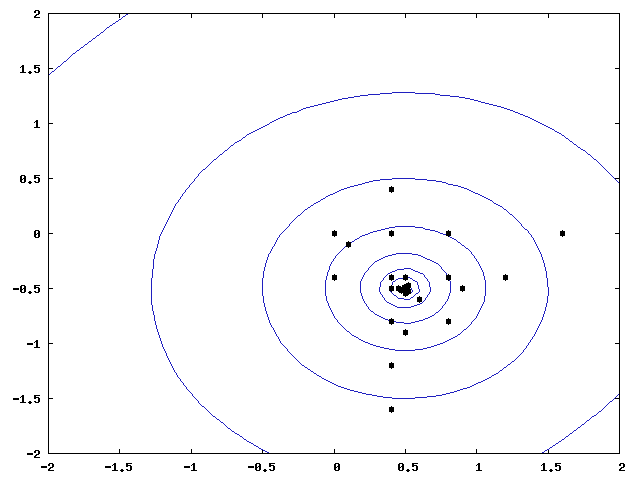
\includegraphics[width=0.5\textwidth]{power}
  \caption{Mesh adaptive direct search evaluation points}
  \label{fig:Power}
\end{figure}

\chapter{Dakota files}

\section{Dakota input file format}

There are six sections in every Dakota input file. These sections are identified with the following keywords: \textit{variables}, \textit{interface}, \textit{responses}, \textit{model}, \textit{method}, and \textit{environment}. At least one \textit{variables}, \textit{interface}, \textit{responses}, and \textit{method} must appear, and no more than one \textit{environment} should appear.

\begin{figure}[htb!]
  \centering
    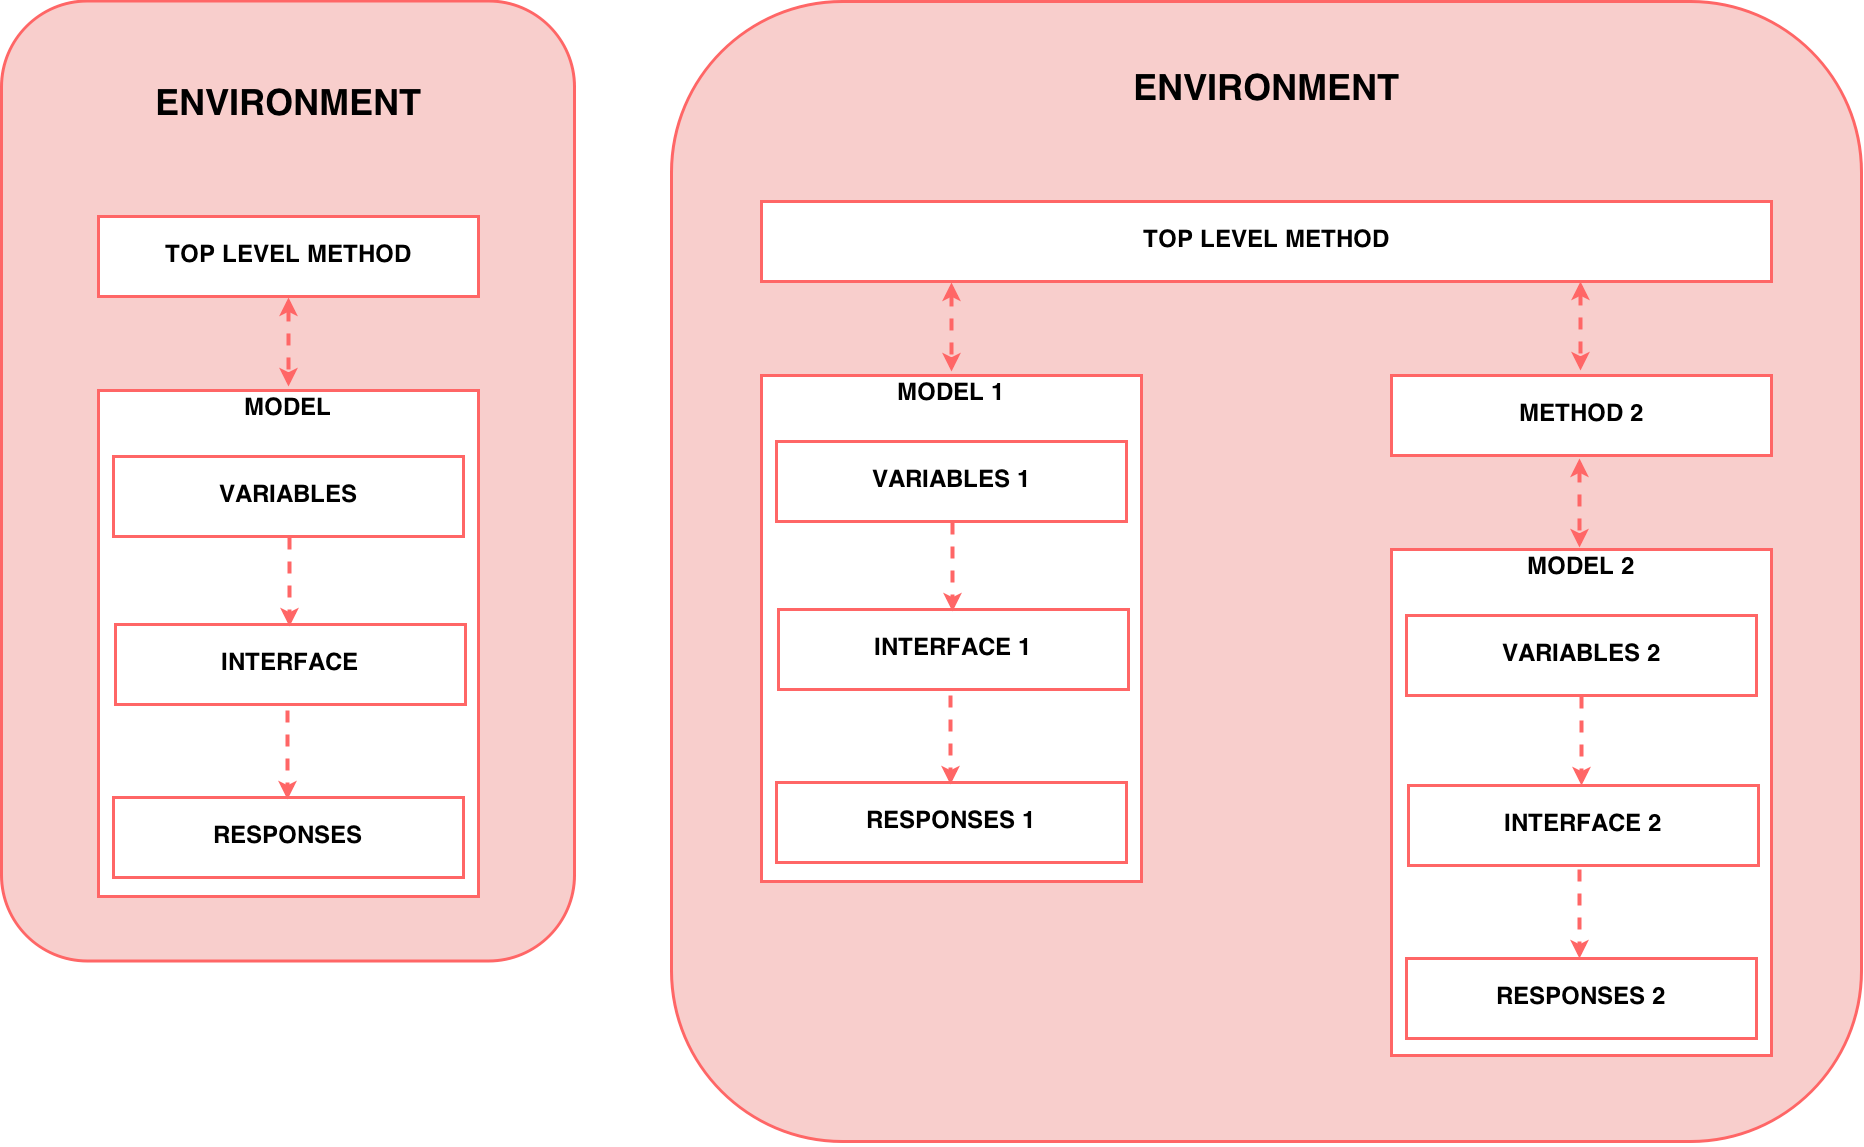
\includegraphics[width=0.8\textwidth]{DakotaInputFile}
  \caption{Relationship between the six blocks}
  \label{fig:InputFile}
\end{figure}

Figure \ref{fig:InputFile} shows the relationships between the six keyword blocks. The environment specifies high level Dakota settings, and identifies the top level method. A method runs a model. A model block defines the connections between variables, the interface, and responses. It shows the most common relationships between blocks but others are possible. Most Dakota analyses just needs to define a single method which runs a single model.

For a more concrete example, a simple Dakota input file, \textit{power\_multidim.in}, for a two-dimensional parameter study on $F(x,y)=(X-0.5)^2+(Y+0.5)^2$ function is shown in Figure \ref{fig:PoMuCode}. This input file will be used to describe the basic format and syntax used in all Dakota input files.

\begin{figure}[htb!]
\begin{lstlisting}[style=MyCodeStyle,language=bash]
environment
  tabular_graphics_data
    tabular_graphics_file = 'power_multidim.dat'

method
  multidim_parameter_study
    partitions = 8 8

model
  single

variables
  continuous_design = 2
    lower_bounds     -2.0     -2.0
    upper_bounds      2.0      2.0
    descriptors       "X"     "Y"

interface
  fork
    analysis_driver = './power.py'
    parameters_file = 'params'
    results_file    = 'results'
    file_save

responses
  response_functions = 1
  no_gradients
  no_hessians
\end{lstlisting}
\caption{File power\_multidim.in}
\label{fig:PoMuCode}
\end{figure}

First, some syntax background:

\begin{itemize}
\item Blocks can follow any order.
\item Comments starts with symbol \textit{\#}.
\item Use of single or double quotes for string inputs.
\item Use of commas and/or white spaces for separation of specifications.
\item The optional use of symbol \textit{=} to indicate supplied data.
\end{itemize}

The first block that we can find in the file is \textit{environment}. This keyword is used to specify the general Dakota settings such as Dakota's graphical output and the tabular data output (via the \textit{tabular\_graphics\_data} keyword).

The \textit{method} block of the input file specifies which iterative method Dakota will employ, such as a parameter study, optimization method, data sampling technique, etc. The keyword \textit{multidim\_parameter\_study} calls for a multidimensional parameter study, while the keyword \textit{partitions} specifies the number of intervals per variable. In this case, there will be eight intervals (nine data points) evaluated between the lower and upper bounds of both variables (bounds provided subsequently in the variables section), for a total of 81 response function evaluations.

The \textit{model} block of the input file specifies the model that Dakota will use. It provides the logical unit for determining how a set of variables is mapped into a set of responses in support of an iterative method. The model allows one to specify a single interface, or to manage more sophisticated mappings involving surrogates or nested iteration. 
Most of the time we are going to use the \textit{single} model, that is the default value for \textit{model} and its definition can be omitted.

The \textit{variables} block of the input file specifies the characteristics of the parameters that will be used in the problem formulation. The variables can be continuous or discrete, and can be classified as design variables, uncertain variables, or state variables. In figure \ref{fig:PoMuCode} you can see as we have defined two continuous design variables, with their upper and lower bounds and a name: X and Y.

The \textit{interface} block of the input file specifies what approach will be used to map variables into responses as well as details on how Dakota will pass data to and from a simulation code. In this example, the keyword \textit{fork} is used to indicate the use of a user-supplied program. Then we find four keywords: 

\begin{itemize}
\item \textit{analysis\_driver:} indicates the name of the program to execute. In this case, it is going to use the python program \textit{power.py}. 
\item \textit{parameters\_file:} name of the Dakota parameters file that the driver would receive from Dakota.
\item \textit{results\_file:} name of the results file that the driver should return to Dakota once it has finished.
\item \textit{file\_save:} It's telling Dakota to not delete parameters and results files once the driver has finished.
\end{itemize}

Dakota will execute the external program like this:

\begin{lstlisting}[style=MyCodeStyle,language=bash]
./power.py params.$i results.$i
\end{lstlisting}

Where \$i is the iteration number of the method.

The \textit{responses} block of the input file specifies the types of data that the interface will return to Dakota. For our example, the assignment \textit{num\_objective\_functions = 1} indicates that there is only one objective function. Since there are no constraints associated with Rosenbrock's function, the keywords for constraint specifications are omitted. The keywords \textit{no\_gradients} and \textit{no\_hessians} indicate that no
derivatives will be provided to the method; none are needed for a parameter study.

\section{Dakota parameters file format}

Prior to invoking a simulation, Dakota creates a parameters file which contains the current parameter values and a set of function requests. Let's execute the same example that we ran in section \ref{section:RunDakota}, but first, uncomment the line that contains \textit{file\_save}. This will prevent Dakota to remove the temporal files that it uses to communicate with the simulation program. If you list your working directory you will see 81 parameters files (params.*) and 81 results files (results.*). This is how it looks like the content of file \textit{params.1}:

\begin{lstlisting}[style=MyCodeStyle,language=bash]
                                          2 variables
                     -2.000000000000000e+00 X
                     -2.000000000000000e+00 Y
                                          1 functions
                                          1 ASV_1:response_fn_1
                                          2 derivative_variables
                                          1 DVV_1:X
                                          2 DVV_2:Y
                                          0 analysis_components
                                          1 eval_id
\end{lstlisting}

This file can be interpreted as a sequence blocks, where every block contains an array.

\begin{itemize}
\item First we find information about variables: the number of variables (2) followed by the variable values and names ($X=-2.0$ and $Y=-2.0$).
\item The second block contains information of the functions: number of functions (1) followed by kind of response. This information is coded in \textit{ASV\_i}. It can be value, gradient and/or Hessian.
\item The third block contains information about active variables.
\item Then information about analysis components.
\item Finally we have an id of the current iteration 
\end{itemize}

\section{Dakota results file format}

Once the simulation code has finished it should return the needed information through a results file. This is the file \textit{results.1}: 

\begin{lstlisting}[style=MyCodeStyle,language=bash]
      8.5 f   
\end{lstlisting}

It returns the function evaluation value. For a general case we will find a line for every requested response, a line for every requested gradient and a line for every requested Hessian.

After a simulation, Dakota expects to read a file containing responses reflecting the current parameters and corresponding to the function requests in the active set vector. The response data must be in proper format. If the amount of data in the file does not match the function request vector, Dakota will abort execution with an error message.

The format of the numeric fields may be floating point or scientific notation. In the latter case, acceptable exponent characters are \textit{E} or \textit{e}.

\chapter{Coupling Alya with Dakota}

Alya is not prepared to read a Dakota parameter file, interpret the data and run the simulation. It cannot generate a Dakota results file. In fact, it probably cannot generate the objective function that we want to optimize. That function may be some kind of combination of the Dakota outputs.

So, If we want to connect Alya simulation code with Dakota we must pre-process Alya inputs and post-process its outputs. In Dakota is very usual to use a bash script to do these steps:

\begin{itemize}
\item Pre-process step: Mix simulation program input files with Dakota parameters file.
\item Simulation step: Run the simulation program.
\item Post process step: Read the needed data from outputs of the simulation, compute a cost function and write the result in the appropriate file.
\end{itemize}

\section{Alya input file preprocessing}

When we run an Alya simulation we will find thousands of parameters in the input files. If we want to run an optimization problem, we must choose the design variables. That means, that the value of that variables can be modified and we must mark those variables in order to be used by Dakota.

In order to mark those variables you should use the same descriptor that you have used in the Dakota input file. For instance, let's imagine that you have a velocity field in one of your Alya input files:

\begin{lstlisting}[style=MyCodeStyle,language=bash]
VELOCITY
	5.0 -4.0 0.0
END VELOCITY  
\end{lstlisting}

If you want to use the two first fields of the velocity as design variables, first you have to create a descriptor for these variables in the Dakota input file:

\begin{lstlisting}[style=MyCodeStyle,language=bash]
variables
  continuous_design = 2
    descriptors     'v_x'     'v_y'
\end{lstlisting}

Then you have to create a template file containing the original Alya input data, but modifying those fields. You should write the descriptor between braces:

\begin{lstlisting}[style=MyCodeStyle,language=bash]
VELOCITY
	{v_x} {v_y} 0.0
END VELOCITY
\end{lstlisting}

This file is ready to be processed with \textbf{dprepro}, which comes with the Dakota distribution. It is an application that can read a Dakota parameter file (variable names and values) and a file supplied by the user (our template file) and generate a file that can be used by our simulation code. Usage:

\begin{lstlisting}[style=MyCodeStyle,language=bash]
dprepro parameters_file template_input_file new_input_file
\end{lstlisting}

If you want to try a simple example:
\begin{itemize}
\item Create a working directory.
\item Copy all files from path \textit{/gpfs/projects/bsc21/DAKOTA/Examples/preproc} to your working directory.
\item Execute: \textit{dprepro params veloc.tmp veloc}
\end{itemize}

If your design variables are stored in different Alya files you will have to create a template file and run dprepro for each one.

\section{Set up Alya execution}

Running one Alya instance for a large problem can consume a lot of resources. Running an optimization problem will require to execute Alya many times. It becomes very important to save these resources as much as possible. We encourage you to use restart files for your executions and to define a proper output set up.

Using a good restart file can speed up your simulation. If the state of the simulation begins close to the solution it will be more stable and it will converge faster.

Right now we are working in prepare a system to use multiple restart files. Our idea is to create some kind of database where we can find restart files associated with evaluation points. Every time that we want to evaluate a new point we must search in the database for the most appropriate restart file. Once our function evaluation has finished we will save a new restart file for future use.

The output from Alya is not necessarily in a shape useful for Dakota, and it can be different for every problem. Alya output can be very large and become a bottleneck, so it's important to focus the attention in the required data. The model solved with Alya must be configured so that all possible desired output is correctly set. Alya provides many options on where on the model output should be stored: volumes, areas, points.

\section{Alya output post-process}

In any case, the output we get is not the cost function expected by Dakota. We need to post-process this information in order to compute the appropriate cost function. We have created a default way in which Alya users can write a script (it can be a simply bash or python script) that reads the Alya output files, computes an externally prepared cost function, and writes the output in the Dakota results file, using the appropriate format.

In path /gpfs/projects/bsc21/DAKOTA/Examples/postpro you will find an example of how to read Alya outputs and Dakota parameters file, compute a cost function and return the result in a Dakota results file. This is the Python code of file \textit{ReactorCost.py}:

\begin{lstlisting}[style=MyCodeStyle,language=Python,numbers=left]
#!/usr/bin/python
import sys
from DKTutils import ProgramError
from DKTutils import AlyaReadSet, DakotaReadParams
######################################
## Main program
######################################

# Part 1: Read script number of parameters
if len(sys.argv) != 4 :
  ProgramError( "Bad number of parameters" )

# Part 2: Read script parameters
p_name = sys.argv[1]   # Alya problem name
d_para = sys.argv[2]   # Dakota parameters file
d_resu = sys.argv[3]   # Dakota results file

# Part 3: Read the Alya boundary file
f_name =p_name+"-boundary.chm.set"
mode   = "last"
# If mode="last" only the last time step is read (alt: all)
Chemic = AlyaReadSet( f_name, mode="last" )

# Part 4: Extract Input flux (SET=2) and Output flux (SET=1)
#         specie:  TG=1, MG=2, DG=3, GL=4, METH=5 and FAME=6
In_flux = Chemic[2][1:]    # Ignore first element.
Ou_flux = Chemic[1][1:]    # Ignore first element.

# Part 5: Read variable values from Dakota parameters file
VARS = DakotaReadParams( d_para )
Vel = VARS["V"]
Tem = VARS["T"]

# Part 6: Compute the cost function
# Price of every specie
SPEC_Price = [ 0.1, 0.11, 0.11, 0.05, 0.1, 0.25 ]
# Number of species
Nspecies  = len(SPEC_Price)

# Compute the benefit from chemical reactions
# WARNING: Output flux is defined positive in Alya
#          Input flux is defined negative
Benefit = 0.0
for j in range(Nspecies) :
  Benefit += SPEC_Price[j]*(Ou_flux[j]+In_flux[j])

# Compute the cost to increment the temperature
CostTem = 1.0e-3*(Tem-300.0)**2

# Compute the cost to increment the speed
CostVel = 2.0e-5*(Vel-0.01)**2

# Total Cost
Cost = CostTem + CostVel - Benefit

# Part 7: Write the result in the output file
f = open(d_resu,"w")
f.write( str(Cost)+ " f\n" )
f.close()
\end{lstlisting}

This is a simple Python script. We have divided it in several parts:
\begin{enumerate}[label=Part \arabic*:,align=right,labelwidth=2.0cm,leftmargin=2.0cm]
\item First we check that we are calling the script with the appropriate number of parameters.
\item We read three parameters:
\begin{itemize}
\item Alya's problem name.
\item Dakota's parameters file name.
\item Dakota's results file name.
\end{itemize}
\item Read the Alya boundary file using function \textit{AlyaReadSet} (it is defined inside file \textit{DKTutils.py}). It returns an structure containing the information of a boundary or a witness point.
\item Extract the needed information of the previous structure. The first dimension of the structure contains the Alya \textit{Set}. The second dimension contains the elements. The third dimension, if required, contains the time steps.
\item Read the values of the Dakota parameters file using function \textit{DakotaReadParams} (this function is also defined in \textit{DKTutils.py}).
\item Compute a cost function. In this example we calculate the following equation:

$CostTem = 1.0\times10^3*(Tem-300.0)^{2}$

$CostVel = 2.0\times10^5*(Vel-0.01)$

$Benefit = \sum\limits_{i=1}^{species} (Cost(i)*(Ou_flux(i)-In_flux(i)))$

$Cost = CostTem + CostVel - Benefit$

\item Finally, it writes the result in an output file using the Dakota format.

\end{enumerate}

If you want a run this example, create a working directory, copy all the files from the example path and run:
\begin{lstlisting}[style=MyCodeStyle,language=bash]
./ReactorCost.py reactor params results
\end{lstlisting}

\section{Alya execution script}

In path /gpfs/projects/bsc21/DAKOTA/Examples/runscript you will find an executable script that couples Dakota with Alya. This is the bash script file \textit{RunAlya.sh}:

\begin{lstlisting}[style=MyCodeStyle,language=bash]
#!/bin/bash

# STEP 1: Process parameters
if [ $# -ne 2 ]; then
  echo "ERROR: wrong number of parameters" 1>&2
  echo "ERROR: $0 + <input_file> + <output_file>" 1>&2
  exit
elif [ ! -f $1 ]; then
  echo "ERROR: Couldn't find  Input File= $1" 1>&2
  echo "ERROR: $0 + <input_file> + <output_file>" 1>&2
  touch $2
  exit 
fi
Input_File=$1
Output_File=$2

# STEP 2: Define variables
TOPDIR=`pwd`
ALYA_EXEC=${HOME}/Projects/Alya/Executables/unix/Alya.x
ALYA_FILES=${TOPDIR}/cavtri03
ALYA_NAME=cavtri03
NUM=$( grep eval_id ${Input_File} | awk '{print $1}' ) # Iter Num
# WORKDIR=$TMPDIR/workdir.${NUM}
WORKDIR=${TOPDIR}/workdir.${NUM}

# STEP 3: Create temporary working directory
if [ -d ${WORKDIR} ]; then rm -rf ${WORKDIR}; fi
  mkdir ${WORKDIR}
cd ${WORKDIR} > /dev/null

# STEP 4: Copy Needed files to the working directory.
cp ${TOPDIR}/${Input_File} .  # Dakota parameters file
ln -s ${ALYA_FILES}/* .       # Symbolic link to Alya input files

# STEP 5: Merge Dakota and Alya files
dprepro ${Input_File} cavtri03.ker.dat.tmp cavtri03.ker.dat

# STEP 6: Run Alya
MPIRUN="mpirun -np 4"
${MPIRUN} ${ALYA_EXEC} ${ALYA_NAME} 2> alya.err > alya.out
stat=$?

# STEP 7: Error processing.
if [ "${stat}" -ne "0" ]; then
  echo "Error in ALYA."  1>&2
  echo "  Error code: ${stat}."  1>&2
  touch ${TOPDIR}/${Output_File}
  exit
fi


# STEP 8: Post-process alya output and write output file
export PYTHONPATH=${TOPDIR}
ln -s ${TOPDIR}/CavtriCost.py .
./CavtriCost.py ${ALYA_NAME} ${Input_File} ${Output_File}

# STEP 9: Copy output file to the top directory
cp ${Output_File} ${TOPDIR}
\end{lstlisting}

The file is divided in steps:

\begin{enumerate}[label=Step \arabic*:,align=right,labelwidth=2.0cm,leftmargin=2.0cm]
\item Check the script input parameters.
\item Define environment variables. It is important to define several variables:
\begin{itemize}
\item Alya executable.
\item Path containing the Alya input files.
\item The name of the Alya problem.
\item The working directory. We use the Dakota iteration number to generate a different path for every execution.
\end{itemize}
\item Create the working directory. Every Alya execution should be done in a new path.
\item Copy required files to the working directory: Dakota parameters file, Alya input files and any other required file.
\item Merge Alya and Dakota files using \textit{dprepro}. Use \textit{dprepro} with every Alya file that requires to be preprocessed.
\item Run Alya. In this example we are running with MPI and four processes. We will explain more sophisticated uses of MPI later.
\item Check if there is an error. We must check if the Alya simulation has reached the desired state. We can parse the Alya error file or the output file to look for error messages or undesired results.
\item Post-process Alya output, compute a cost function and write the result in a Dakota results file. If there is an error we can try to modify any of the Alya parameters or create an empty output file. This will stop Dakota execution.
\item Move the results file to the top directory. We must be very careful creating this file. Dakota starts to read the file once this is created. So, it's a bad idea to create the file and then write the results. This can lead to Dakota errors. The best idea is to create the file in a different directory and then move it to the Dakota execution path.
\end{enumerate}

If you want to test this example copy all files to a working directory, modify the environment variables from \textit{RunAlya.sh} and run:

\begin{lstlisting}[style=MyCodeStyle,language=bash]
./RunAlya.sh params.1 results.1
\end{lstlisting}

This will create a new directory, \textit{workdir.1}, that contains the Alya execution and a Dakota results file, \textit{results.1}, that contains the results of the cost function.

\chapter{Running in parallel}
If we run Alya with Dakota we will have multiple levels of parallelism. In one hand, we have Alya, that is a massive parallel program, that can run in serial or in parallel. In the other hand, we have Dakota that sometimes can execute more than one function evaluation at a time. You can choose the method that fits you best:

\begin{itemize}

\item One Alya parallel execution.

From the point of view of Dakota this task is sequential. Dakota doesn't care if our applications uses MPI or OpenMP. Dakota runs only one function evaluation at a time and keeps waiting for a results file to run a new function evaluation.

In path \textit{/gpfs/projects/bsc21/DAKOTA/Examples/parall\_s\_p} you can find of an example of a Dakota multidimensional parameter study of an Alya simulation. This example makes a two dimensional study calling Alya in parallel using the bash script \textit{AlyaRun.sh}.

To run this example, copy all files (including subdirectories) to a local path, edit environment variables from \textit{AlyaRun.sh} and run:

\begin{lstlisting}[style=MyCodeStyle,language=bash]
dakota parall_s_p.in -o parall_s_p.out > parall_s_p.stdout
\end{lstlisting}

This will execute 16 Alya evaluations, one after the other. Everyone in parallel, using 4 MPI processes.


\item Multiple Alya serial executions.

There are some Dakota methods that can evaluate multiple points at the same time. For instance, in a multidimensional parameter study every function evaluation is independent from all the others. We can specify to Dakota how many function evaluations we want to do in parallel.

In order to run multiple task with Dakota you have to include the \textit{asynchronous} keyword inside the \textit{interface} block. You can also set the number of concurrent jobs that can be executed by specifying it through the \textit{evaluation\_concurrency} keyword. For example:

\begin{lstlisting}[style=MyCodeStyle,language=bash]
interface
  fork
    asynchronous
	  evaluation_concurrency = 4
    analysis_driver = './RunAlya.sh'
    parameters_file = 'params'
    results_file    = 'results'
    file_save
\end{lstlisting}

This is setting Dakota to execute 4 instances of \textit{RunAlya.sh} at the same time.

In path \textit{/gpfs/projects/bsc21/DAKOTA/Examples/parall\_p\_s} you will find an example of a Dakota problem running multiple instances of serial Alya executions. It is the same problem that we have seen in the previous point, but with two main differences:
\begin{description}
\item[parall\_p\_s.in] We have added \textit{asynchronous} and \textit{evaluation\_concurrency}.
\item[RunAlya.sh] Variable \textit{MPIRUN} is undefined. So, we will run Alya in serial mode.
\end{description}

\item Multiple Alya parallel executions.

This is a combination of the previous cases. We can run multiple function evaluations running Alya in parallel.

You can find an example in \textit{/gpfs/projects/bsc21/DAKOTA/Examples/parall\_p\_p}. In this example we have activated asynchronous in the Dakota input file and MPI is also enabled in the Alya execution script.

\end{itemize}

\section{Running multiple task in Marenostrum}

If we want to run Dakota in Marenostrum using multiple nodes we can find several problems. Marenostrum has a queue system that allows us to execute one task in a group of processors. It give us a bunch of resources that we will use during our application execution. If we run Dakota, it creates multiple task. We have to distribute these resources between the task.

We can find several scenarios:
\begin{itemize}
\item \textbf{All the resources to one Dakota function evaluation:}
This is the simplest case. We can only execute one instance of Alya at the same time. So we can dedicate all the resources to this function evaluation. It is necessary to find out how many available resources do we have. In our Alya execution script we can add this code:

\begin{lstlisting}[style=MyCodeStyle,language=bash]
# Check if we are in queue system
if [ -n "$LSB_DJOB_HOSTFILE" ] &&     # Exist the variable
   [ -f "$LSB_DJOB_HOSTFILE" ]; then  # Exist the file
  HFILE=$LSB_DJOB_HOSTFILE
  NP=$LSB_DJOB_NUMPROC
elif [ -f hfile ]; then
  HFILE=hfile             # Use a local file as host file
  NP=$( wc -l ${HFILE} | awk '{print $1}' )
else
  HFILE=./.hfile; echo localhost > $HFILE
  NP=$( grep -e "core id" -e "physical id" /proc/cpuinfo |
        sed '$!N;s/\n/ /' | sort -u | wc -l )
fi
MPIRUN="mpirun -hostfile ${HFILE} -np ${NP}"
\end{lstlisting}

These bash commands detects if we are running in the queue system of Marenostrum and uses all available resources to set up MPI. This can be done reading the environment variables \textit{LSB\_DJOB\_HOSTFILE} and \textit{LSB\_DJOB\_NUMPROC}. Otherwise, if we are running in an interactive shell, it looks for a host file provided by the user (\textit{hfile}). If this file does not exist, it will use all the available processors from current node.

You can find an example in path \textit{/gpfs/projects/bsc21/DAKOTA/Examples/LSB.case.1}. Copy all files to a working directory. Edit file \textit{RunAlya.sh} and set the Alya executable path to the desired value. In this directory you will find a queue bash script: \textit{LSBqueues.sh}. You can use this file to execute in the three available modes:

\begin{enumerate}
\item Execute in the current node:
\begin{lstlisting}[style=MyCodeStyle,language=bash]
./LSBqueues.sh
\end{lstlisting}

\item Using a hostfile created by us:
\begin{lstlisting}[style=MyCodeStyle,language=bash]
printf "localhost\nlocalhost\nlocalhost\nlocalhost\n" >  hfile
./LSBqueues.sh
\end{lstlisting}

\item Launching the script to the queue system:
\begin{lstlisting}[style=MyCodeStyle,language=bash]
bsub < LSBqueues.sh
\end{lstlisting}
\end{enumerate}

\item \textbf{Distribute the resources in function of concurrency:}
If a Dakota problem has set the concurrency parameter, we should distribute the available resources. In order to do this, we should check the available resources in the current execution before running Dakota. We must create groups of resources. The number of groups is equal to the number of concurrent executions set in Dakota.

Once our Dakota problem is running there must be a system that controls the access to the different groups. Every new execution should search free resources and lock them, in order that the other execution can't use them.

In path \textit{/gpfs/projects/bsc21/DAKOTA/Examples/LSB.case.2} you can find an example of a Dakota problem with concurrent executions that distribute the available resources. There you will find the file \textit{LSBqueues.sh}.

\begin{lstlisting}[style=MyCodeStyle,language=bash]
#!/bin/bash
#
#  Submit jobs in MN-III  
#     bsub < LSBqueues.sh
#
#
#BSUB -J DakotaRun 
#BSUB -W 00:02
#BSUB -n 32
#BSUB -oo LSBqueues.out
#BSUB -eo LSBqueues.err
#BSUB -q bsc_case

# STEP 1: Set variables
DAKOTA_INP=concurrent.in
DAKOTA_OUT=${DAKOTA_INP%.*}.out
DAKOTA_STD=${DAKOTA_INP%.*}.stdout

# STEP 2: Get available resources
if [ -n "$LSB_DJOB_HOSTFILE" ] &&     # Exist the variable
   [ -f "$LSB_DJOB_HOSTFILE" ]; then  # Exist the file
  HFILE=$LSB_DJOB_HOSTFILE
  NP=$LSB_DJOB_NUMPROC
elif [ -f $./hfile ]; then
  HFILE=./hfile               # Use a local file as host file
  NP=$( wc -l ${HFILE} | awk '{print $1}' )
else
  NP=$( grep -e "core id" -e "physical id" /proc/cpuinfo |
        sed '$!N;s/\n/ /' | sort -u | wc -l )
  HFILE=./.hfile
  for i in $( seq 1 $NP ); do echo localhost; done > $HFILE
fi

# STEP 3: Get CONC from Dakota input file
EV_CONC=$( grep evaluation_concurrency ${DAKOTA_INP} )
CONC=1
if [ ! -z "${EV_CONC}" ]; then
  arr=($EV_CONC)
  NW=${#arr[@]}
  for i in $( seq 1 $NW )
  do
    word1=${arr[i-1]}
    if [[ ${word1} == evaluation_concurrency ]]; then
      word2=${arr[i]}
      if [[ ${word2} == "=" ]]; then
        CONC=${arr[i+1]}; break
      elif [[ ${word2} == "="* ]]; then
        CONC=${word2:1}; break
      else
        CONC=${word2}; break
      fi
    elif [[ ${word1} == "evaluation_concurrency=" ]]; then
      CONC=${arr[i]}; break
    elif [[ ${word1} == "evaluation_concurrency="* ]]; then
      CONC=${s##*=}; break
    fi
  done
fi

# STEP 4: Create a locks directory
LOCKS=.locks
if [ -d $LOCKS ]; then rm -rf .locks; fi
mkdir $LOCKS

# STEP 5: Distribute hosts between concurrent processes
Ini=1
Rem=$NP
CPUSxP=$((NP/CONC))
REST=$((NP%CONC))
for i in $( seq ${CONC} )
do
  if [ $i -le $REST ]; then
    End=$((Ini+CPUSxP))
  else
    End=$((Ini+CPUSxP-1))
  fi
  fname=$( printf "hfile.%03d" $i )
  sed  -n "$Ini,$End p" < $HFILE > $LOCKS/$fname
  Ini=$(($End+1))
done

# STEP 6:
dakota -i ${DAKOTA_INP} -o ${DAKOTA_OUT} > ${DAKOTA_STD}
\end{lstlisting}

This is a bash script that can be used to run Dakota in Marenostrum queue system. It is divided in several steps:
\begin{enumerate}[label=Step \arabic*:,align=right,labelwidth=2.0cm,leftmargin=2.0cm]
\item Set Dakota input file name and other variables.
\item Get the available resources.
\item Parse the Dakota input file to extract the concurrency of the problem.
\item Create a temporary directory to contain the lock files.
\item Divide the main host file in as many pieces as concurrent jobs. We get smaller host files.
\item Run Dakota.
\end{enumerate}

Then, we have also modified the Alya execution script, \textit{RunAlyaCon.sh}. We have added this new step:

\begin{lstlisting}[style=MyCodeStyle,language=bash]
# STEP 6.1: Get a host file and create a lock
for file in $( ls ${TOPDIR}/.locks/hfile.??? )
do
  LOCK_DIR=${file}.d
  if mkdir ${LOCK_DIR} 2> /dev/null ; then
    HFILE=${file}
    break
  fi
done
NP=$( wc -l ${HFILE} | awk '{ print $1 }' )
MPIRUN="mpirun -hostfile ${HFILE} -np ${NP}"
\end{lstlisting}

In order to create a log we use the instruction \textit{mkdir}. This is an atomic instruction. If we succeed creating the directory, it means that we can get that host file. Otherwise, we should look for another file. Once we have finished we must release the lock:

\begin{lstlisting}[style=MyCodeStyle,language=bash]
# STEP 10: Release lock
rm -rf ${LOCK_DIR}
\end{lstlisting}

\item \textbf{Ask for more resources every time that we need to execute a new task:} In this scenario we are going to ask for new resources every time that Dakota executes the Alya execution script. Alya execution and post-process is encapsulated inside an LSF script that is generated and submitted to the queue system.

You can find an example in path \textit{/gpfs/projects/bsc21/DAKOTA/Examples/LSB.case.3}. There, you can find file \textit{RunAlyaQueue.sh}. This is the interesting part of the file:

\begin{lstlisting}[style=MyCodeStyle,language=bash]
# STEP 6: Create an LSF file
cat << EOF > ${QUEUE_FILE}
#BSUB -J DakotaRun 
#BSUB -W ${QUEUE_TIME}
#BSUB -n ${QUEUE_NODES}
#BSUB -oo ${QUEUE_FILE%.*}.out
#BSUB -eo  ${QUEUE_FILE%.*}.err
#BSUB -q bsc_case

mpirun ${ALYA_EXEC} ${ALYA_NAME} 2> alya.err > alya.out
stat=\$?

# STEP 7: Error processing.
if [ "\${stat}" -ne "0" ]; then
  echo "Error in ALYA."  1>&2
  echo "  Error code: \${stat}."  1>&2
  touch ${TOPDIR}/${Output_File}
  exit
fi

# STEP 8: Post-process alya output and write output file
export PYTHONPATH=${TOPDIR}
ln -s ${TOPDIR}/CavtriCost.py .
./CavtriCost.py ${ALYA_NAME} ${Input_File} ${Output_File}

# STEP 9: Copy output file to the top directory
cp ${Output_File} ${TOPDIR}
EOF

# STEP 10: Submit the script to the Queue system
chmod +x ${QUEUE_FILE}
bsub < ${QUEUE_FILE}

# STEP 11: Wait until the file is created
while [ ! -f ${TOPDIR}/${Output_File} ]; do sleep 1; done
\end{lstlisting}

Steps 6 to 10 are encapsulated inside an script. In step 10 we submit the script to the queue system. In the last step we wait until the  output file is created.

If you want to run this example, you should modify some environment variables in this file. Note, that you can set how many processors your Alya simulation will use and its time limit. You should run:
\begin{lstlisting}[style=MyCodeStyle,language=bash]
bsub < LSBqueues.sh
\end{lstlisting}

\end{itemize}
 
Using one method or the other will depend on the problem and the available resources. With the first method we are losing one level of parallelism, but we are not wasting resources. With the second method we can run more than one Alya execution at the same time, but we can waste resources. Some times it is not possible to execute more than one Alya execution at the same time, some resources will be unused. The third method works in parallel and does not waste resources, but introduces a delay. We have to wait for the queue system to give us a new slot for every execution. This can be very annoying because it depends on Marenostrum load.

\chapter{Dakota methods}

\section{Parameter study capabilities}
Dakota parameter studies explore the effect of parametric changes within simulation models by computing response data sets at a selection of points in the parameter space, yielding one type of sensitivity analysis. The selection of points is deterministic and structured, or user-specified, in each of the four available parameter study methods:

\begin{description}
\item[Vector] Performs a parameter study along a line between any two points in an n-dimensional parameter space, where the user specifies the number of steps used in the study.

To use this method you must specify an initial point:

\begin{lstlisting}[style=MyCodeStyle,language=bash]
variables
  continuous_design = M
    initial_point     (vector of M reals)
\end{lstlisting}

and a final point with a number of steps:

\begin{lstlisting}[style=MyCodeStyle,language=bash]
method
  vector_parameter_study
    final_point       (vector of N reals)
    num_steps         ( integer )
\end{lstlisting}

or an step size and the number of steps:

\begin{lstlisting}[style=MyCodeStyle,language=bash]
method
  vector_parameter_study
    step_vector       (vector of M reals)
    num_steps         ( integer )
\end{lstlisting}

In path \textit{/gpfs/projects/bsc21/DAKOTA/Examples/PaStVector}, you can find an example of every case. You can use \textit{vectorFP.in} and \textit{vectorSV.in} as Dakota input files.

\item[List] The list parameter study computes response data sets at selected points in parameter space. These points are explicitly specified by the user.

In order to use this method, you must specify a list of points:

\begin{lstlisting}[style=MyCodeStyle,language=bash]
method,
	list_parameter_study,
	list_of_points =  (point 1)
	                  (point 2)
	                  ...
	                  (point N)
\end{lstlisting}

or a file containing a list of points:

\begin{lstlisting}[style=MyCodeStyle,language=bash]
method,
	list_parameter_study,
	import_points_file =  points_file
\end{lstlisting}

In the \textit{/gpfs/projects/bsc21/DAKOTA/Examples/PaStList} directory, you can find a Dakota example of each of the cases (\textit{listOfPo.in} and \textit{listPoFi.in}). You can also find an example of how to write a points file (\textit{PointsFile.dat}. These files should use this structure:

\begin{lstlisting}[style=MyCodeStyle,language=bash]
% Comment line / Description of the columns
       1     EMPTY           ( Vector of N reals 1 )
       2     EMPTY           ( Vector of N reals 2 )
       ...
       M     EMPTY           ( Vector of N reals M )
\end{lstlisting}

\item[Centered] The centered parameter study executes multiple coordinate-based parameter studies, one per parameter, centered about the specified Initial Values. This is useful for investigation of function contours in the vicinity of a specific point. For example, after computing an optimum design, this capability could be used for post-optimality analysis in verifying that the computed solution is actually at a minimum or constraint boundary and in investigating the shape of this minimum or constraint boundary.

You must specify an initial point, and a step size and a number of steps in each direction:

\begin{lstlisting}[style=MyCodeStyle,language=bash]
variables
  continuous_design = N
    initial_point = ( Vector of N floats )

method
  centered_parameter_study
    step_vector         ( Vector of N floats )
    steps_per_variable  ( Vector of N integers )
\end{lstlisting}

In path \textit{/gpfs/projects/bsc21/DAKOTA/Examples/PaStCenter}, you can find a Dakota input file example: \textit{CenterPar.in}.

\item[Multidimensional] The multidimensional parameter study computes response data sets for an n-dimensional hypergrid of points. Each variable is partitioned into equally spaced intervals between its upper and lower bounds, and each combination of the values defined by these partitions is evaluated.

You must specify an upper and a lower bound for every direction, and the number of partitions that we will need for every variable:

\begin{lstlisting}[style=MyCodeStyle,language=bash]
variables
  continuous_design = N
    lower_bounds      ( Vector of N floats )
    upper_bounds      ( Vector of N floats )

method
  multidim_parameter_study
    partitions        ( Vector of N integers )
\end{lstlisting}

In path \textit{/gpfs/projects/bsc21/DAKOTA/Examples/PaStMultid}, you can find a Dakota input file example: \textit{MultiPar.in}.
\end{description}

\section{Optimization methods}
\subsection{Gradient-Based Local Methods}
Gradient-based optimizers are best suited for efficient navigation to a local minimum in the vicinity of the initial point. They are not intended to find global optima in nonconvex design spaces. Gradient-based optimization methods are highly efficient, with the best convergence rates of all of the local optimization methods, and are the methods of choice when the problem is smooth, unimodal, and well-behaved.

Gradient accuracy is a critical factor for gradient-based optimizers, as inaccurate derivatives will often lead to failures in the search or pre-mature termination of the method. Analytic gradients and Hessians are ideal but often unavailable. It is most often the case for engineering applications, however, that a finite difference method will be used by the optimization algorithm to estimate gradient values. You can set Dakota to compute finite differences modifying the \textit{responses} block:

\begin{lstlisting}[style=MyCodeStyle,language=bash]
responses
  objective_functions = 1
  no_gradients
  numerical_gradients              # Use finite difference
    method_source dakota           # Use Dakota bounds
    interval_type central          # central/forward diff
    fd_gradient_step_size = 1.e-4  # Step of the difference
  no_hessians
\end{lstlisting}

Note, that, for optimization problems, we ask for objective functions instead of response functions. If our Alya simulation can compute derivatives we can set our Dakota input file using the keyword: \textit{analytic\_gradients}.

Gradient-based methods for nonlinear optimization problems can be described as iterative processes in which a sequence of subproblems, usually which involve an approximation to the full nonlinear problem, are solved until the solution converges to a local optimum of the full problem. The optimization methods available in Dakota fall into several categories, each of which is characterized by the nature of the subproblems solved at each iteration:

\begin{description}

\item[Conjugate gradient] methods require first derivative information and can only be applied to unconstrained problems. The subproblems entail minimizing a quadratic function over a space defined by the gradient and directions
that are mutually conjugate with respect to the Hessian, though the Hessian is never computed. There are several variants of how those directions are defined. There are several methods available in Dakota: \textit{conmin\_frcg}, \textit{dot\_frcg} (not available) and \textit{optpp\_cg}.

In path \textit{/gpfs/projects/bsc21/DAKOTA/Examples/OpConjGrad} you will find an example of optimizing an Alya problem using the conmin algorithm (\textit{conmin.in}).

\item[Sequential Quadratic Programming (SQP)] methods are appropriate for nonlinear optimization problems with nonlinear constraints. Each subproblem involves minimizing a quadratic approximation the Lagrangian subject to linearized constraints. Only gradient information is required; Hessians are approximated by low-rank updates defined by the step taken at each iterations. Dakota has three SQP methods (\textit{dot\_sqp}, \textit{nlpql\_sqp} and \textit{npsol\_sqp}), but they are not available because the required libraries are not installed.

\item[Newton Methods] can be applied to nonlinear optimization problems with nonlinear constraints. The subproblems associated with these methods entail finding the solution to a linear system of equations derived by setting the derivative of a second-order Taylor series expansion to zero. We can find several versions:

\begin{itemize}
\item The full Newton method (\textit{optpp\_newton}) expects both gradients and Hessians to be provided.
\item Quasi-Newton methods (\textit{optpp\_q\_newton}, \textit{dot\_bfgs}) expect only gradients. The Hessian is approximated by the Broyden-Fletcher-Goldfarb-Shanno (BFGS) low-rank updates.
\item The finite difference Newton method (\textit{optpp\_fd\_newton}) expects only gradients and approximates the Hessian with second-order finite differences.
\end{itemize}

In path \textit{/gpfs/projects/bsc21/DAKOTA/Examples/OpNewtonMe} you can find three examples that use Newton methods with an Alya optimization problem: \textit{optpp\_newton.in},  \textit{optpp\_q\_newton.in} and \textit{optpp\_fd\_newton.in}.

\item[Method of Feasible Directions] (MFD) methods are appropriate for nonlinear optimization problems with nonlinear
constraints. These methods ensure that all iterates remain feasible. Dakota includes conmin\_mfd and dot\_mmfd.

\end{description}

\subsection{Derivative-Free Local Methods}

Derivative-free methods can be more robust and more inherently parallel than gradient-based approaches. They can be applied in situations were gradient calculations are too expensive or unreliable. In addition, some derivativefree methods can be used for global optimization which gradient-based techniques, by themselves, cannot. For these reasons, derivative-free methods are often go-to methods when the problem may be nonsmooth, multimodal, or poorly behaved. It is important to be aware, however, that they exhibit much slower convergence rates for finding an optimum, and as a result, tend to be much more computationally demanding than gradientbased methods. Given the computational cost, it is often prudent to use derivative-free methods to identify regions of interest and then use gradient-based methods to home in on the solution.

There are several derivative-free methods available in Dakota:

\begin{description}
\item[Pattern search] methods can be applied to nonlinear optimization problems with nonlinearities. There are three  pattern search methods available in Dakota that vary according to richness of available stencil and the way constraints supported: \textit{asynch\_pattern\_search}, \textit{coliny\_pattern\_search} and \textit{mesh\_adaptive\_search}.

In path \textit{/gpfs/projects/bsc21/DAKOTA/Examples/OpPatSe} you can find two examples of how to run a pattern search method: \textit{mesh.in} and \textit{asynch.in}.

\item[Simplex] methods for nonlinear optimization problem are similar to pattern search methods, but their search directions are defined by triangles that are reflected, expanded, and contracted across the variable space. The two simplex-based methods available in Dakota are optpp\_pds and coliny\_cobyla. These methods can not run multiple task at the same time.

\item[Greedy Search Heuristic] for nonlinear optimization problems is captured in the Solis-Wets (coliny\_solis\_wets) method. This method takes a sampling-based approach in order to identify search directions. It does a poor job solving problems with nonlinear constraints and it can not run multiple tasks
\end{description}


\subsection{Derivative-Free Global Methods}
There are two types of global optimization methods in Dakota:

\begin{description}
\item[Evolutionary Algorithms] (EA) are based on Darwin’s theory of survival of the fittest. The EA algorithm starts with a randomly selected population of design points in the parameter space, where the values of the design parameters form a “genetic string,” analogous to DNA in a biological system, that uniquely represents each design point in the population. The EA then follows a sequence of generations, where the best design points in the population (i.e., those having low objective function values) are considered to be the most “fit” and are allowed to survive and reproduce. The EA simulates the evolutionary process by employing the mathematical analogs of processes such as natural selection, breeding, and mutation. Ultimately, the EA identifies a design point (or a family of design points) that minimizes the objective function of the optimization problem. EAs available in Dakota include \textit{coliny\_ea}, \textit{soga}, and \textit{moga}.

\item[DIvision of RECTangles (DIRECT)] balances local search in promising regions of the design space with global search in unexplored regions. It adaptively subdivides the space of feasible design points to guarantee that iterates are generated in the neighborhood of a global minimum in finitely many iterations. Dakota includes two implementations (\textit{ncsu\_direct} and \textit{coliny\_direct}).

In path \textit{/gpfs/projects/bsc21/DAKOTA/Examples/OpDivRec} you can find file \textit{ncsu.in} that implements an optimization using \textit{ncsu\_direct} method.

\item[Efficient Global Optimization (EGO)] is a global optimization technique that employs response surface surrogates. In each EGO iteration, a Gaussian process (GP) approximation for the objective function is constructed based on sample points of the true simulation. The GP allows one to specify the prediction at a new input location as well as the uncertainty associated with that prediction. The key idea in EGO is to maximize an Expected Improvement Function (EIF), defined as the expectation that any point in the search space will provide a better solution than the current best solution, based on the expected values and variances predicted by the GP model. Points with good expected values and even a small variance will have a significant expectation of producing a better solution (exploitation), but so will points that have relatively poor expected values and greater variance (exploration). This provides a balance between exploiting areas of the design space that predict good solutions, and exploring areas where more information is needed.

In path \textit{/gpfs/projects/bsc21/DAKOTA/Examples/OpEGO} you can find an example of efficient global optimization: \textit{EGO.in}.

\end{description}

\subsection{Optimization with User-specified or Automatic Scaling}

Some optimization problems involving design variables, objective functions, or constraints on vastly different scales may be solved more efficiently if these quantities are adjusted to a common scale (typically on the order of unity). With any optimizer, user-specified characteristic value scaling may be applied to any of continuous design variables, functions/residuals, nonlinear inequality and equality constraints, and linear inequality and equality constraints. Automatic scaling is available for variables or
responses with one- or two-sided bounds or equalities and may be combined with user-specified scaling values. Logarithmic (log10) scaling is available and may also be combined with characteristic values. Log scaling is not available for linear constraints. Moreover, when continuous design variables are log scaled, linear constraints are not permitted in the problem formulation. Discrete variable scaling is not supported.

Scaling is enabled by including the \textit{scaling} keyword in the relevant method specification in the Dakota input deck. When scaling is enabled the values are transformed such that the optimizer iterates in scaled variable space, whereas evaluations of the computational model as specified in the interface are performed on the original problem scale.

Scaling for a particular variable or response type is enabled through the \textit{*\_scale\_types} specification. Valid options
for this string specification include \textit{`none'} (default), \textit{`value'}, \textit{`auto'}, or \textit{`log'}, for no, characteristic value, automatic, or logarithmic scaling, respectively.

The user may additionally specify no, one, or a vector of characteristic scale values through the \textit{*\_scales} specification. These characteristic values are ignored for scaling type \textit{`none'}, required for \textit{`value'}, and optional for \textit{`auto'} and \textit{`log'}.

\appendix

\chapter{Dakota Source code modification}
\label{chapter:CodeMod}

Original code from Dakota has an incompatibility with the queue system of Marenostrum. The queue system kills all the asynchronous task that Dakota uses to run concurrent jobs. We have modified Dakota code to avoid this problem.

In the Linux Bash terminal, an orphan process can be created by attaching an ampersand at the end of the command line. This is an abstract of the original file CommandShell.cpp where we can see how Dakota runs asynchronous jobs:

\begin{lstlisting}[style=MyCodeStyle,language=C++]
CommandShell& CommandShell::flush()
{
  if (asynchFlag)
    sysCommand += " &";
  std::system(sysCommand.c_str());
}
\end{lstlisting}

As we can see, Dakota makes a system call using the ampersand when the asynchronous flag is true. In this case, the new process is orphan and this can became a problem. If we want to avoid this, we can not use the ampersand.

\begin{lstlisting}[style=MyCodeStyle,language=C++]
CommandShell& CommandShell::flush()
{
  if (asynchFlag)
  {
    if ( fork() == 0 )
    {
      std::system(sysCommand.c_str());
      exit( 0 );
    }
  }
  else
    std::system(sysCommand.c_str());
}
\end{lstlisting}

In the new version, we call fork to create a new Dakota process for each new simulation. We can identify the original process because the returning value of fork is different from zero. This process exits the function without doing anything. Meanwhile, the new process (its returning value from fork is equal to zero) makes the system call to execute the task, but without detaching it. The task is never an orphan process. Once the task is finished the process is terminated.

\end{document}
